\documentclass[10pt,a4paper]{article}
\usepackage[T1]{fontenc}
\usepackage[utf8]{inputenc}
\usepackage{lmodern,microtype}
\usepackage[margin=15mm,top=14mm,bottom=15mm]{geometry}
\usepackage{amsmath,booktabs,tabularx,array,xcolor,graphicx,caption,fancyhdr,hyperref}

\definecolor{navy}{HTML}{16324F}
\definecolor{blue}{HTML}{2563A6}
\definecolor{green}{HTML}{047857}
\definecolor{red}{HTML}{B42318}
\definecolor{amber}{HTML}{A05A00}
\definecolor{lightblue}{HTML}{EAF2FA}
\definecolor{lightgray}{HTML}{F2F4F7}
\hypersetup{colorlinks=true,linkcolor=blue,urlcolor=blue}
\graphicspath{{latex/}}
\pagestyle{fancy}
\fancyhf{}
\lhead{\scriptsize\color{navy}\textbf{Forecast adaptation and TS-IFA}}
\rhead{\scriptsize\color{gray}Results through 7 August 2026}
\cfoot{\scriptsize\color{gray}\thepage}
\renewcommand{\headrulewidth}{0.3pt}
\setlength{\headheight}{13pt}
\setlength{\parindent}{0pt}
\setlength{\parskip}{3pt}
\captionsetup{font=small,labelfont={bf,color=navy},skip=3pt}
\newcolumntype{Y}{>{\raggedright\arraybackslash}X}
\newcolumntype{C}{>{\centering\arraybackslash}X}
\newcommand{\code}[1]{\texttt{\detokenize{#1}}}
\newcommand{\gain}[1]{\textcolor{green}{+#1\%}}
\newcommand{\loss}[1]{\textcolor{red}{#1\%}}
\newcommand{\sectionbar}[1]{\vspace{2pt}{\large\bfseries\color{navy}#1}\par\vspace{2pt}\color{black}}
\newcommand{\callout}[1]{\colorbox{lightblue}{\parbox{0.965\linewidth}{\small #1}}}

\begin{document}
{\huge\bfseries\color{navy}Retrieval-based forecast adaptation}\par
{\Large\color{blue}Executive summary of results}\par
\vspace{5pt}

\callout{\textbf{Evaluation basis.} Screen and ablation averages weight equally
the 12 held-out T3 dataset/window configurations (Electricity, Traffic, Solar,
Exchange Rate; three $(L,H)$ settings). Gains are nMSE improvements over the
vanilla forecast; positive is better.}

\sectionbar{Decision snapshot}
\small
\begin{tabularx}{\linewidth}{@{}p{31mm}Yp{45mm}@{}}
\toprule
\textbf{Question} & \textbf{Quantitative answer} & \textbf{Decision} \\
\midrule
Best baseline? & Shared full ridge, instance-space, reaches
\gain{2.733} at $K=3$ in the screen and \gain{2.991} at $K=10$ in the
$K$ sweep. & Retain the vanilla-anchored ridge family. \\
Best gate? & Best screen gate: \gain{0.019}; best gate ablation:
\gain{0.045}; diagnostic oracle: up to \gain{13.34}. & Current learned gates
do not capture the available oracle headroom. \\
Convex or $\Delta$? & Mean over six matched designs: ridge \gain{2.427},
$\Delta$-ridge \gain{1.251}, convex \gain{0.783}. & Both constraints remain
positive but are dominated by ordinary ridge. \\
Does TS-IFA work? & The 10K ridge run reaches only \gain{0.04} on T3; 30K
ridge fits fall to \loss{-6.71} and \loss{-17.97}. & No robust success; select
on the fixed T2 criterion and stop earlier. \\
\bottomrule
\end{tabularx}

\sectionbar{Best average baselines and gates}
\begin{tabularx}{\linewidth}{@{}Yp{25mm}p{24mm}r@{}}
\toprule
\textbf{Method} & \textbf{Retrieval} & \textbf{Evidence set} &
\textbf{Mean T3 gain} \\
\midrule
Shared full ridge correction & instance, $K=10$ & $K$ sweep & \gain{2.991} \\
Shared context--future ridge correction & instance, $K=20$ & $K$ sweep & \gain{2.954} \\
Shared future--forecast ridge correction & instance, $K=20$ & $K$ sweep & \gain{2.861} \\
Shared full ridge correction & instance, $K=3$ & primary screen & \gain{2.733} \\
\midrule
Per-horizon Bayes context gate & instance, $K=1$ & gate ablation & \gain{0.045} \\
Shared CatBoost neighbour-average gate & instance, $K=3$ & primary screen & \gain{0.019} \\
Shared CatBoost context gate & instance, $K=1$ & primary screen & \gain{0.015} \\
Shared neighbour-average oracle & instance, $K=3$ & diagnostic oracle & \gain{13.34} \\
\bottomrule
\end{tabularx}

\sectionbar{Winning formulas, written out}
\footnotesize
Let $V_h$ be the vanilla forecast, $C_h$ the context forecast, $Y_{k,h}$ the
$k$th neighbour's observed future, $N_{k,h}$ its backbone forecast, and
$\bar Y_h=\sum_k w_kY_{k,h}$. The shared coefficients below are fitted by ridge
to the correction target $Y_h-V_h$ and are common to every horizon:
\[
\begin{aligned}
\widehat Y_h^{\mathrm{full}}&=V_h+\beta_VV_h+\beta_CC_h+
 \sum_{k=1}^{K}(\beta^Y_kY_{k,h}+\beta^N_kN_{k,h}),\\
\widehat Y_h^{\mathrm{context+future}}&=V_h+\beta_VV_h+\beta_CC_h+
 \sum_{k=1}^{K}\beta^Y_kY_{k,h},\\
\widehat Y_h^{\mathrm{future+forecast}}&=V_h+\beta_VV_h+
 \sum_{k=1}^{K}(\beta^Y_kY_{k,h}+\beta^N_kN_{k,h}).
\end{aligned}
\]
For the best gate, $\widehat Y_h=C_h$ exactly when the T1+T2 mean of
$(Y_h-V_h)^2-(Y_h-C_h)^2$ is positive, otherwise $\widehat Y_h=V_h$.
The shared CatBoost gates use $\widehat Y_h=A_h$ when
$g_\theta(z)>0$, otherwise $V_h$, where $A\in\{\bar Y,C\}$ and $g_\theta$
regresses the mean squared-error reduction from $V$ to $A$.

\newpage
\sectionbar{Formulation ablations}
\small
\begin{tabularx}{\linewidth}{@{}Yrrr@{}}
\toprule
\textbf{Matched feature design} & \textbf{Ridge} & \textbf{$\Delta$-ridge} &
\textbf{Convex} \\
\midrule
Full $(C,Y_{1:K},N_{1:K})$ & 2.733\% & 1.515\% & 0.635\% \\
$Y_{1:K}$ & 2.293\% & 1.347\% & 1.209\% \\
$C+Y_{1:K}$ & 2.546\% & 1.468\% & 1.115\% \\
$Y_{1:K}+N_{1:K}$ & 2.539\% & 1.339\% & 0.330\% \\
$C+\bar Y$ & 2.306\% & 1.183\% & 1.063\% \\
$C$ & 2.142\% & 0.652\% & 0.347\% \\
\midrule
\textbf{Mean over designs} & \textbf{2.427\%} & \textbf{1.251\%} &
\textbf{0.783\%} \\
Mean loss versus matched ridge & -- & $-1.176$ pp & $-1.643$ pp \\
\bottomrule
\end{tabularx}

\vspace{4pt}
\sectionbar{Effect of the neighbour count $K$}
\begin{center}
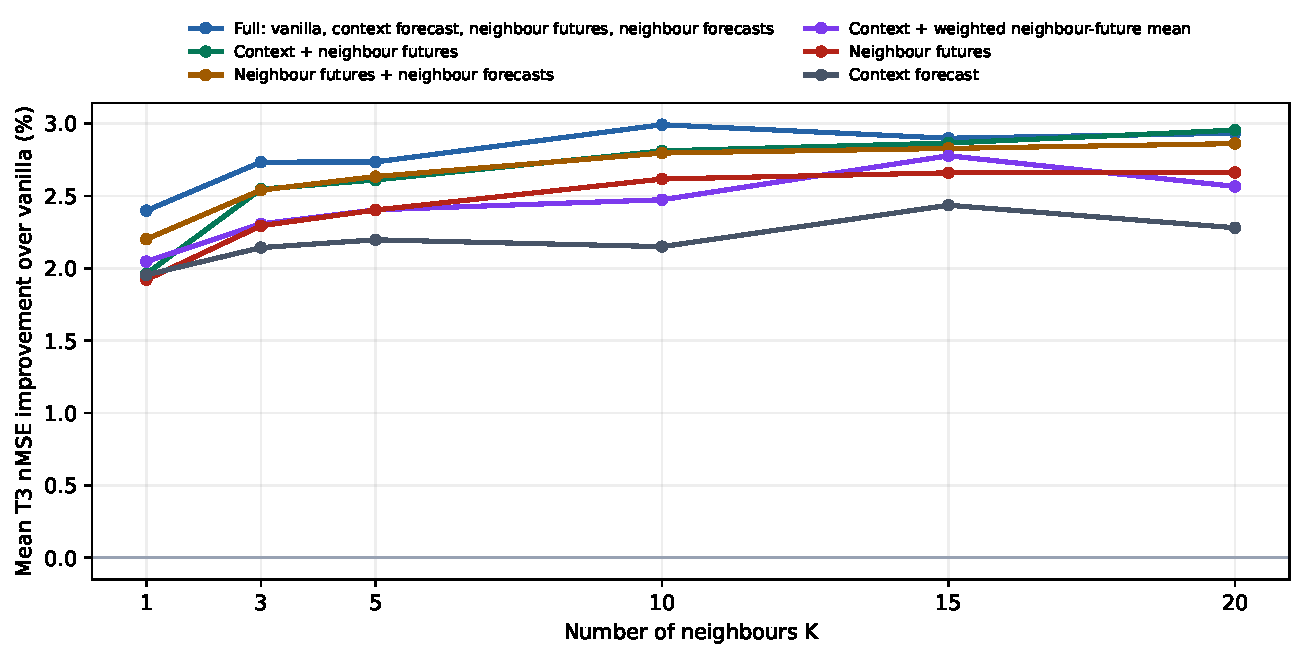
\includegraphics[width=0.97\linewidth]{k_ablation_ridge_curves.pdf}
\captionof{figure}{Mean held-out T3 nMSE improvement over 12 configurations.
Only ridge baselines are shown: most improve from $K=1$ toward $K=10$--20,
with no common optimum across feature designs.}
\end{center}

\footnotesize
\begin{tabularx}{\linewidth}{@{}YcrYc@{}}
\toprule
\textbf{Ridge} & \textbf{Best $K$} & \textbf{Gain} & \textbf{Ridge} &
\textbf{Best $K$ / gain} \\
\midrule
Full & 10 & 2.991\% & $C+Y$ & 20 / 2.954\% \\
Residual & 20 & 2.861\% & $C+\bar Y$ & 15 / 2.777\% \\
$Y$ & 20 & 2.661\% & $C$ & 15 / 2.435\% \\
\bottomrule
\end{tabularx}

\newpage
\sectionbar{TS-IFA results}
\small
\begin{tabularx}{\linewidth}{@{}YrrY@{}}
\toprule
\textbf{Run} & \textbf{T2 gain} & \textbf{T3 gain} &
\textbf{Checkpoint / held-out behaviour} \\
\midrule
Joint ridge, raw, 10K & +1.84\% & +0.04\% & Window gains
$+3.26,+0.58,-3.72$\%; all three select 10K. \\
Joint ridge, raw, 30K & +3.03\% & $-6.71$\% & Selected at
$29/20/20$K for $(168/24,336/48,504/168)$. \\
Joint ridge, instance, 30K & +3.25\% & $-17.97$\% & Selected at
$30/26/20$K for the same windows. \\
Joint neural, raw / instance, 30K & -- & $-4.60/-2.14$\% & Zero T3 wins. \\
\bottomrule
\end{tabularx}

\begin{center}
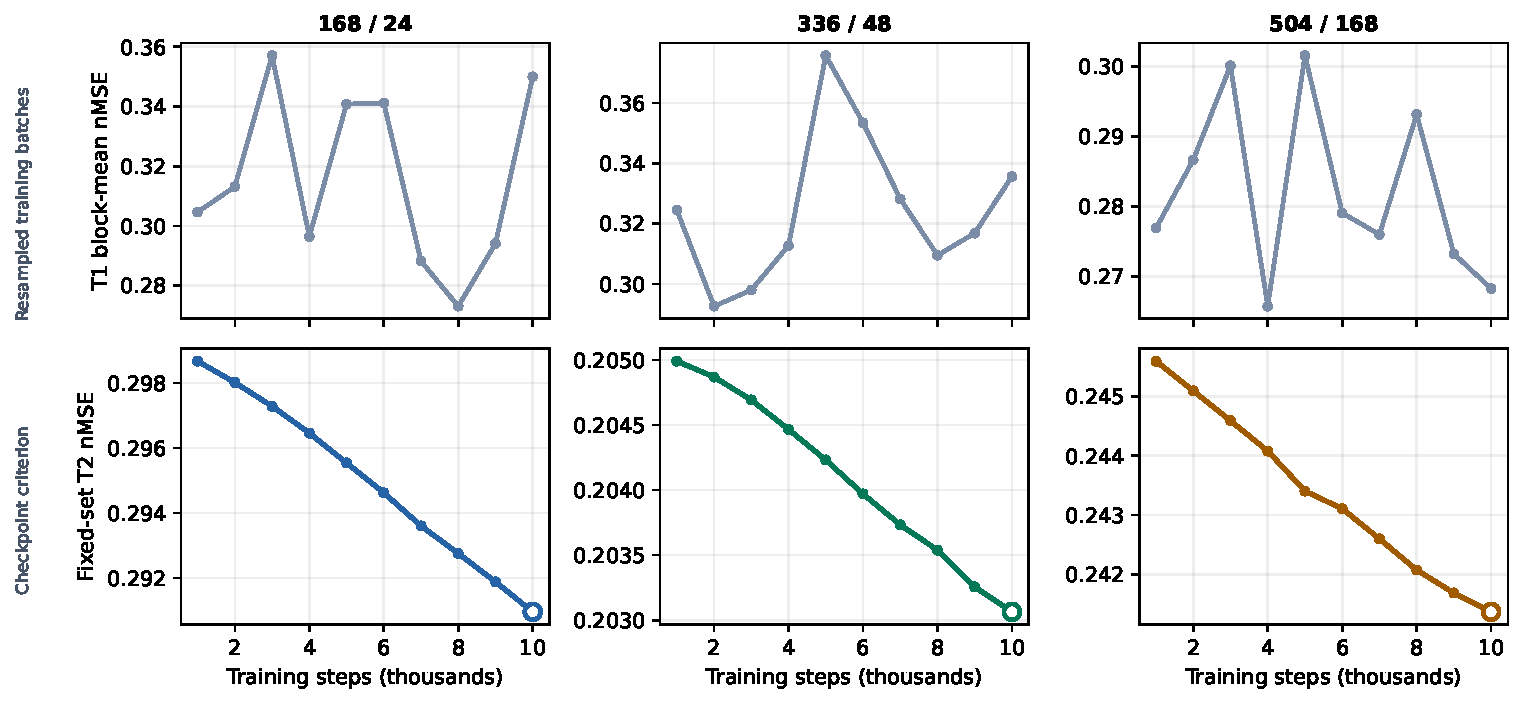
\includegraphics[width=0.98\linewidth]{ts_ifa_10k_criterion_curves.pdf}
\captionof{figure}{The 10K joint-ridge criterion curves. The gray T1 trace is a
1,000-step block mean over freshly resampled training batches, not a repeated
evaluation on one fixed set, so it need not be monotone. The colored T2 trace
uses a fixed set and selects 10K for all three windows.}
\end{center}

\callout{\textbf{Answer.} TS-IFA does not yet work reliably. The 30K runs
generalize worse than the 10K run. Four of six ridge fits select their best T2
checkpoint at 20--26K, while the two $168/24$ fits select 29--30K; better T2
selection still does not translate to T3.}

\sectionbar{Decisions before reruns}
\footnotesize
\begin{tabularx}{\linewidth}{@{}p{34mm}Y@{}}
\toprule
\textbf{Retain} & \textbf{Reason supported above} \\
\midrule
Ridge candidates & Reproduce the $K=3$ screen and test $K=10,15,20$ with the
same held-out evaluation. \\
Gate diagnostics & Retain hard CatBoost/Bayes gates and oracles to measure the
unclosed 13.34\% diagnostic gap. \\
TS-IFA & Re-run with explicit T2 early stopping and untouched T3; include the
10K checkpoint and continue only while the fixed-set T2 criterion improves. \\
\bottomrule
\end{tabularx}

\vfill
{\scriptsize\color{gray}Source: screen, CatBoost, convex, delta, $K$ and TS-IFA
results. Percentages are equal-weight means of per-setting nMSE improvement
over vanilla; positive is better. Target-aware oracles are diagnostic only.}
\end{document}
